
\begin{frame}{Recap \& Refresh}

        \begin{itemize}
		\item Why going Bayesian? \textit{p}-values are troublesome.
		\item Theorem: $p({\theta}|{y}) = \frac{f({y}|{\theta})\pi({\theta})}{\int f({y}|{\theta}) \pi({\theta})  d{\theta}}$
		\item Normal-Normal model: $p(\theta|y) = N(\theta|\frac{\sigma^2\mu+\tau^2y}{\sigma^2+\tau^2},\frac{\sigma^2\tau^2}{\sigma^2 + \tau^2})$
        	\item Monte Carlo sampling        
        \end{itemize}

\end{frame}

\begin{frame}{Intended Learning Outcomes}

        At the end of this day you will be able to:
        \begin{itemize}
                \item describe the pros and cons of using different priors (e.g. elicited,
                conjugate, ...);
                \item evaluate the interplay between prior and posterior distributions using \texttt{R},
                \item calculate several quantities of interest from posterior distributions,
                \item apply Bayesian inference to estimate population variation from DNA data.
        \end{itemize}

\end{frame}

\begin{frame}{Prior distributions}

	How can we decide which prior distribution is more appropriate in our study?
	\begin{itemize}
		\item They are derived from past information or personal opinions from experts.
		\item They are typically distributed as commonly used distribution families.
		\item They can be limited to to bear little information.
		\item ...endless possibilities...
	\end{itemize}

\end{frame}

\begin{frame}{Elicited priors}

	\begin{block}{}
		\begin{itemize}
			\item Define the collection of $\theta$ which are \textit{possible},
			\item assign some probability to each one of these cases,
			\item make sure that they sum up to $1$.
		\end{itemize}
	\end{block}

\end{frame}

\begin{frame}{Elicited \textbf{discrete} priors}

	\begin{figure}[ht]
		\centering
		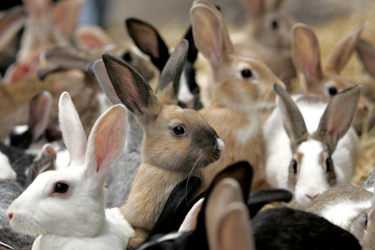
\includegraphics[width=4cm]{Images/Rabbits.jpeg}
		\caption{How many kits do rabbits have in one litter?}
	\end{figure}

	Knowing that "rabbits can have anywhere from one to 14 babies in one litter with an 
	average litter size of 6", let's build a prior distribution.

\end{frame}

\begin{frame}{Elicited \textbf{continuous} priors}

	\begin{figure}[!ht]
		\centering
		\includegraphics[width=4cm]{Images/BumpassHell.jpeg}
		\caption{Bumpass Hell, hot springs and fumaroles at Lassen Volcanic National Park, California.}
	\end{figure}

	Knowing that "from past observations, the temperature has a range of (80.1, 110.4) with an 
	average of 88.3 Celsius degrees", let's build a prior distribution.

\end{frame}

\begin{frame}{Elicited \textbf{parametric} priors}

	$\theta$ belongs to a parametric distributional family $\pi(\theta|\nu)$.

	Advantages:
	\begin{itemize}
		\item reduces the effort to the elicitee,
		\item overcomes the finite support problem,
		\item may lead to simplifications in the computation of the posterior.
	\end{itemize}

	Disadvantage:
	\pause
	\begin{itemize}
		\item impossible to find a distribution that perfectly matches the elicitee's beliefs.
	\end{itemize}

\end{frame}

\begin{frame}{Elicited \textbf{parametric} priors}

	\begin{equation}
		\begin{displaystyle}
			\pi(\theta) = 
			\begin{cases}
				0 & \text{for } \theta < 80.1 \text{ or } \theta > 110.4 \\
				N(\mu,\sigma^2) & \text{for } 80.1 \leq \theta \leq 110.4     
			\end{cases}
		\end{displaystyle}
	\end{equation}
	with $\mu=88.3$ and $\sigma^2=10$

	\begin{figure}[!ht]
		\centering
		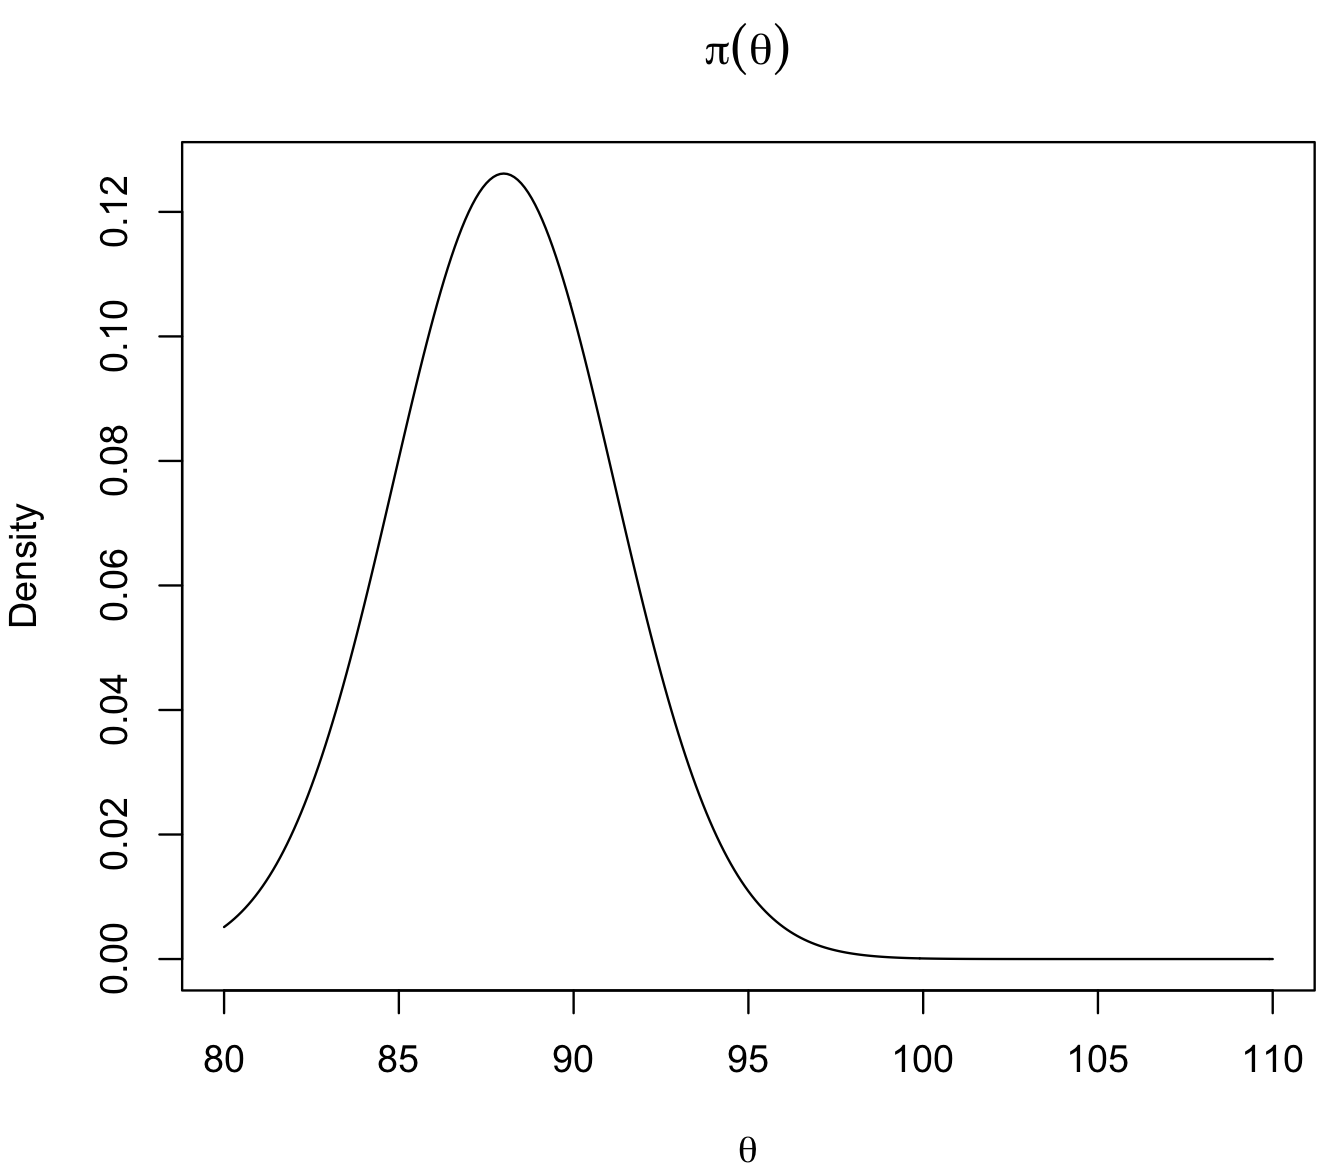
\includegraphics[width=4.5cm]{Figures/PriorLassen.png}
		\caption{Elicited prior distribution of water temperature.}
	\end{figure}

\end{frame}

\begin{frame}{How to build elicited priors}

	\begin{itemize}
		\item Focus on quantiles close to the middle of the distribution (e.g. the $50^{th}$, 
		$25^{th}$ and $75^{th}$) rather than extreme quantiles (e.g. the $95^{th}$ and $5^{th}$),
		\item assess the symmetry,
		\item priors can be updated and reassessed as new information is available,
		\item useful for experimental design and data exploration.
	\end{itemize}

\end{frame}

\frame{
\frametitle{Conjugate priors}

	\begin{block}{}
		$\pi(\theta)$ is member of a family which is \textit{conjugate} with the likelihood $f({y}|\theta)$ 
		so that the posterior distribution $p(\theta|{y})$ belongs to the same distributional family as the prior.
	\end{block}

}

%%%%%%%%%%%%%%%%%%%%%%%%%%%%%%%%%%

\frame{
\frametitle{Conjugate priors}

Example: $Y$ is the count of distinct elephant herds arriving at the pool in a day during the migration season.

\begin{figure}[!ht]
\centering
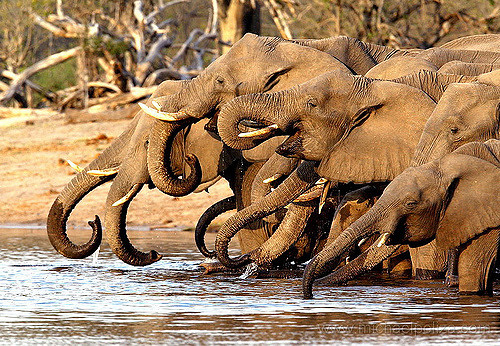
\includegraphics[width=4cm]{Images/Elephants.jpeg}
\caption{Elephants drinking at the pool. What's the arrival rate for distinct herds?}
\label{Fig:Elephants}
\end{figure}

}

%%%%%%%%%%%%%%%%%%%%%%%%%%%%%

\frame{
\frametitle{Poisson and elephants}

Poisson distribution is an appropriate model for $Y$ if:
\begin{enumerate}
\item $Y$ is the number of times an event occurs in an interval and it can take values any positive integer values including 0;
\item the occurrence of one event does not affect the probability that a second event will occur (i.e. events occur independently);
\item the rate at which events occur is constant (it cannot be higher in some intervals and lower in other intervals);
\item two events cannot occur at exactly the same instant;
\item the probability of an event in an interval is proportional to the length of the interval.
\end{enumerate}

}

%%%%%%%%%%%%%%%%%%%%

\frame{
\frametitle{Poisson distribution}

If $\theta$ is the event rate (rate parameter), then the probability of observing $y$ events in an interval is:
\begin{equation}
f(y|\theta) = \frac{e^{-\theta}\theta^y}{y!} \text{, } y \in \{0, 1, 2, ...\} \text{, } \theta>0
\end{equation}
which is the probability mass function (pmf) for a Poisson distribution.

\vskip 1cm

Let's plot the distribution for $\theta=4$ using \texttt{R}.

}

%%%%%%%%%%%%%%%%%%%%%%%

\frame{
\frametitle{Poisson distribution}

\begin{figure}[!ht]
\centering
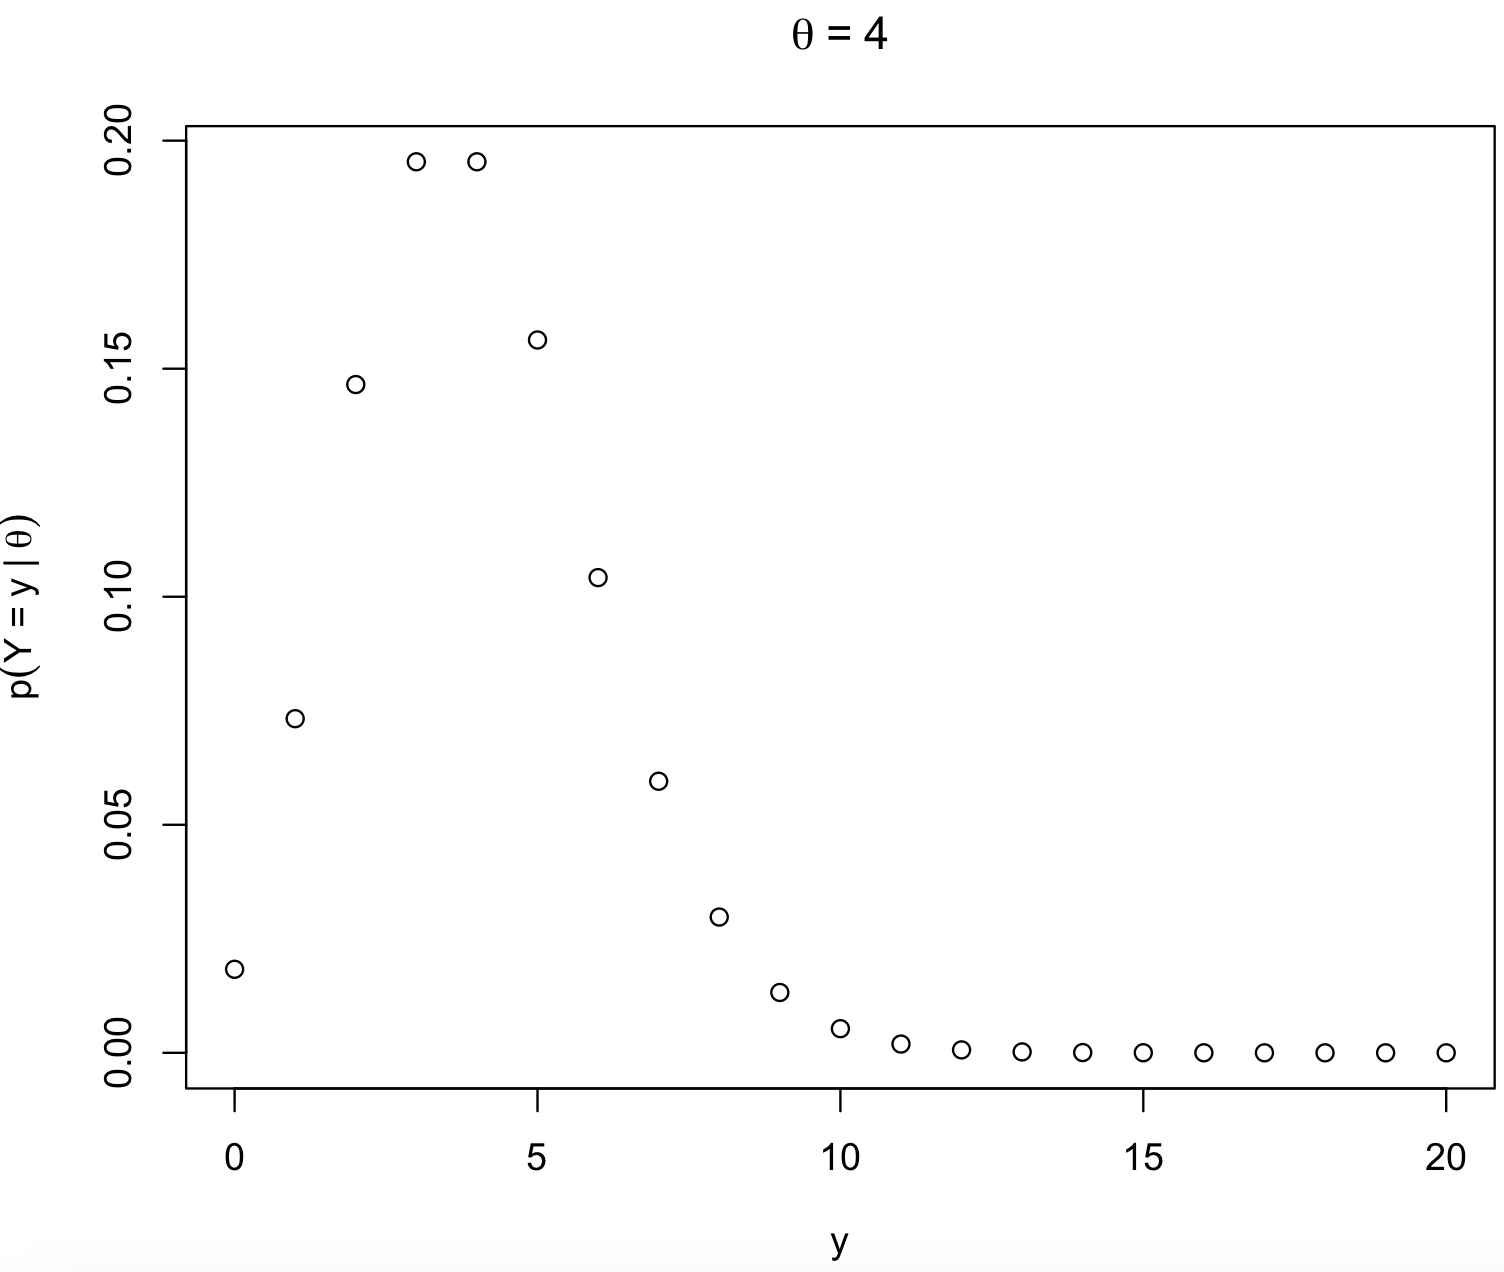
\includegraphics[width=5cm]{Figures/PoissonLike.png}
\caption{Poisson distribution for $\theta=4$. This is the likelihood distribution for the number of herds per day with a rate of 4.}
\end{figure}

}

%%%%%%%%%%%%%%%%%%%%%%%

\frame{
\frametitle{Conjugate prior for Poisson distribution}

Prior: Gamma distribution

\begin{equation}
\pi(\theta) = \frac{\theta^{\alpha-1}e^{-\theta/\beta}}{\Gamma(\alpha)\beta^\alpha} \text{, } \theta>0 \text{, } \alpha>0 \text{, } \beta>0
\end{equation}

\begin{align}
E[G(\alpha,\beta)] &= \alpha\beta\\                                     
Var[G(\alpha,\beta)] &= \alpha\beta^2
\end{align}

}


%%%%%%%%%%%%%%%%%%%%%%

\frame{
\frametitle{Gamma distribution}

\begin{figure}[!ht]
\centering
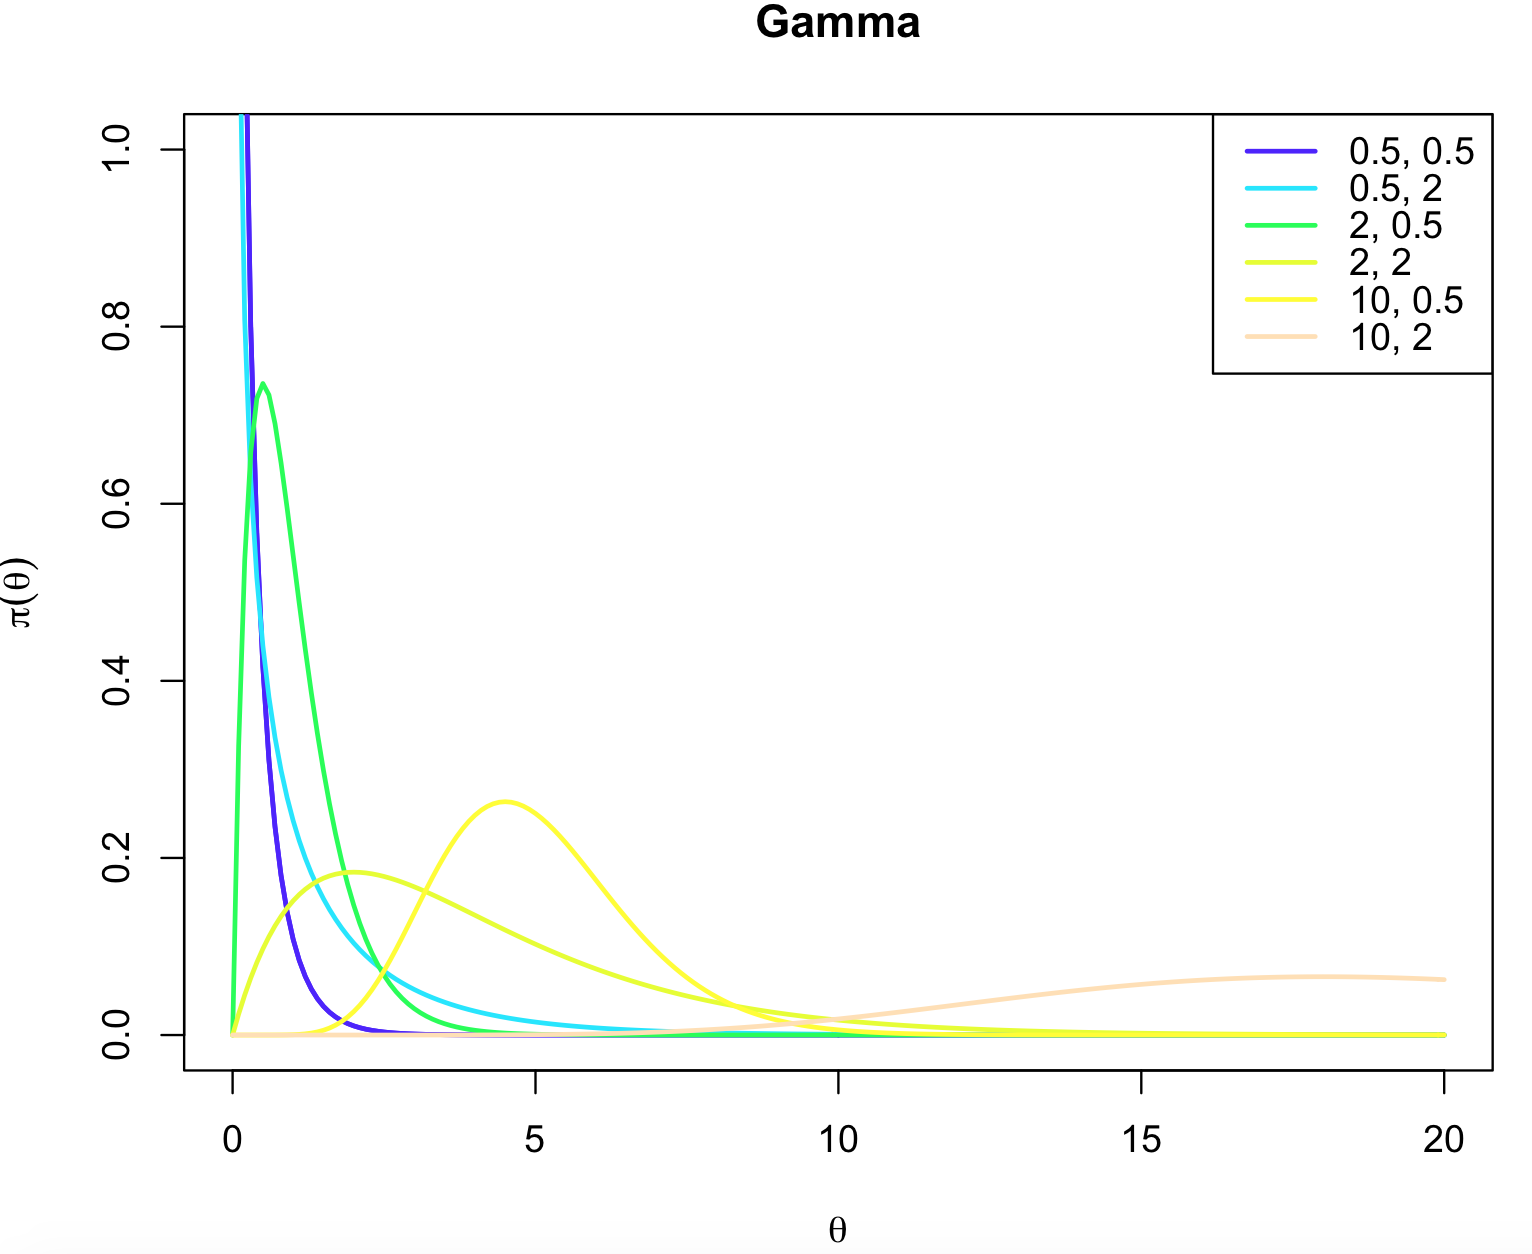
\includegraphics[width=6cm]{Figures/GammaPrior.png}
\caption{Gamma distribution for different values of shape and rate parameters.}
\label{Fig:Gamma}
\end{figure}

}

%%%%%%%%%%%%%%%%%%%%%%%

%%%%%%%%%%%%%%%%%%%%%%%

\frame{
\frametitle{Gamma + Poisson = ?}

\begin{align}
p(\theta|y) &\approx f(y|\theta) \pi(\theta)\\
&\approx ?
\end{align}

}

\frame{
\frametitle{Gamma + Poisson = Gamma'}

\begin{align}
p(\theta|y) &\approx f(y|\theta) \pi(\theta)\\
&\approx (e^{-\theta}\theta^y)(\theta^{\alpha-1}e^{-\theta/\beta})\\
&= \theta^{y+\alpha-1}e^{-\theta(1+1/\beta)}
\end{align}

$p(\theta|y) ~ \sim G(\alpha',\beta')$ with $\alpha'=y+\alpha$ and $\beta'=(1+1/\beta)^{-1}$

Posterior is (another) Gamma distribution.

\begin{block}{}
Conjugate priors allow for posterior distributions to emerge without numerical integration!
\end{block}

}

%%%%%%%%%%%%%%%%%%%%%%%

\frame{
\frametitle{Elephants' arrivals}

Example:
\begin{itemize}
\item we have some intuition that we expect to see 3 herds per day (prior)
\item we observed 4 herds (data)
\end{itemize}

\vskip 1cm

Exercise:\\
What is the posterior distribution of $\theta$, the average number of herds (Gamma-Poisson model)?
Calculate and plot the distribution in \texttt{R} (use Monte Carlo sampling too).


}

\frame{
\frametitle{Hierarchical modelling}

\textit{Hyperpriors} define the density distribution of hyperparameters.
\begin{equation}
	p({\theta}|{y}) = \frac{ \int f({y}|{\theta})\pi({\theta}|{\nu})h({\nu})d{\nu} }{ \int \int  f({y}|{\theta})\pi({\theta}|{\nu})h({\nu})d{\nu}d{\theta} } 
\end{equation}

\pause

\begin{block}{Empirical Bayesian}
\textit{Estimated posterior} $p({\theta}|{y},\hat{{\nu}})$ by replacing ${\nu}$ with an estimate $\hat{{\nu}}$ obtained by maximising the marginal distribution $m({y}|{\nu})$.
\end{block}

If ${\nu} \sim h({\nu}|{\lambda})$ with unknown parameters ${\lambda}$, then we have a third-stage prior $g({\lambda})$.

}

%%%%%%%%%%%%%%%%%%%%%%%

\frame{
\frametitle{Non-informative priors}

Can we use a Bayesian approach when no reliable prior information on ${\theta}$ is available?

Yes, a \textit{noninformative prior} distribution for ${\theta}$ contains "no information" about ${\theta}$ and all the information in the posterior will (mostly) arise from the data.


}

%%%%%%%%%%%%%%%%%%%%%%%

\frame{
\frametitle{Noninformative priors}

Discrete case:

If $\vec{\Theta}=\{\theta_1, \theta_2, ..., \theta_n\}$, then
\begin{equation*}
p(\theta_i) = \frac{1}{n} \text{, } i=1, 2, ...,n 
\end{equation*}
with
\begin{equation*}
\sum_1^n \frac{1}{n}=1 
\end{equation*}

}


\frame{
\frametitle{Noninformative priors}

Continuous and bounded case:

If $\vec{\Theta}=[a,b]$ with $-\infty<a<b<+\infty$, then
\begin{equation*}
p(\theta) = \frac{1}{b-a} \text{, } a<\theta<b
\end{equation*}

}

%%%%%%%%%%%%%%%%%%%%%%%

\frame{
\frametitle{Noninformative priors}

Continuous and unbounded case:

If $\vec{\Theta}=(-\infty,+\infty)$ then
\begin{equation*}
p(\theta) = c \text{, any } c>0 
\end{equation*}
is an \textit{improper} distribution as
\begin{equation*}
\int_{-\infty}^{+\infty} p(\theta) d\theta = +\infty 
\end{equation*}

Bayesian inference is still possible under some circumstances.

}

%%%%%%%%%%%%%%%%%%%%%%%

\frame{
\frametitle{Noninformative priors}

\begin{figure}[!ht]
\centering
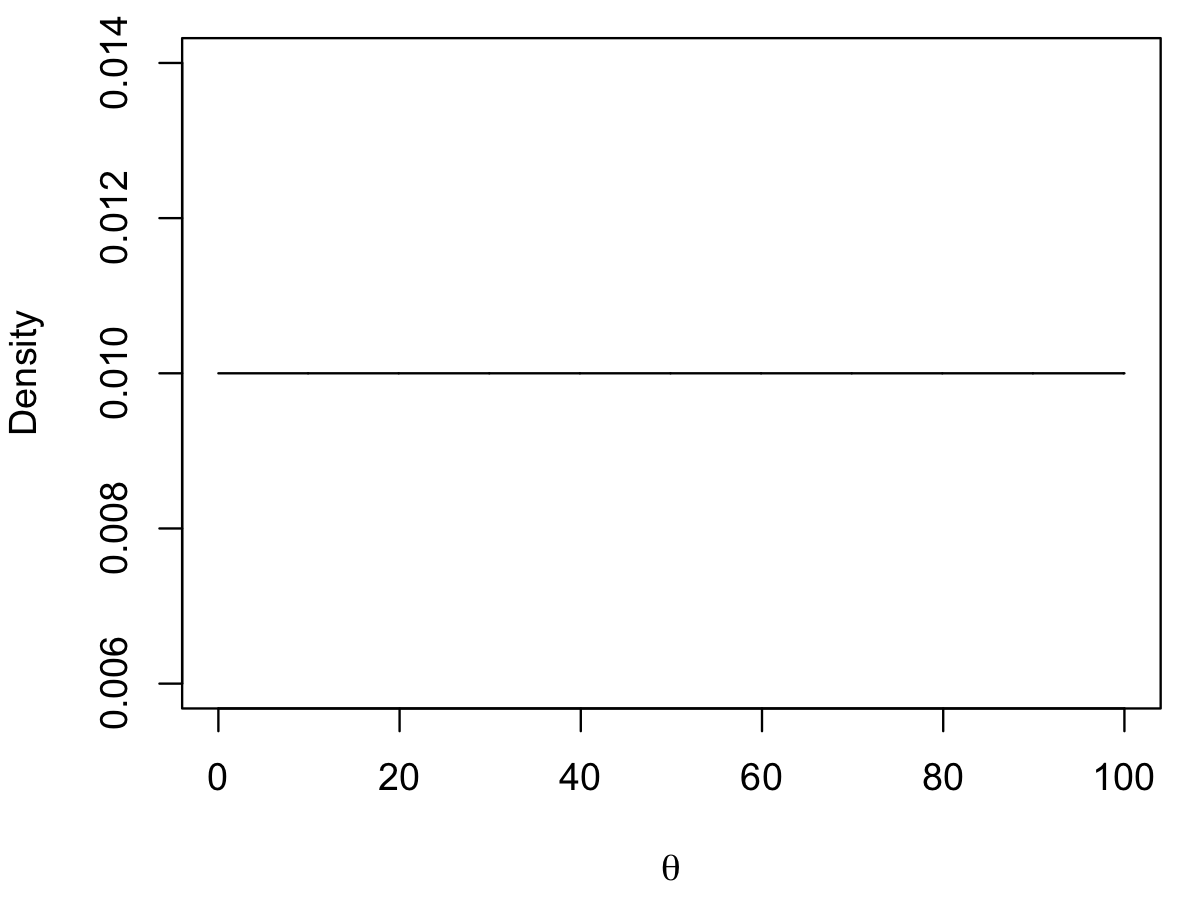
\includegraphics[width=4cm]{Figures/Uniform.png}
\caption{A uniform prior distribution for the arrival rate of elephant herds.}
\label{Fig:Uniform}
\end{figure}

\begin{itemize}
\item Rule out scenarios that are impossible in real life.
\item Lack a conjugate model (sampling methods are required).
\item Non-informative priors are related to \textit{reference} priors.
\end{itemize}

}



